	\subsection{Taxonomy of virtualization technologies by \textit{Pessolani}}
	
	\begin{figure}[H]
		\centering
		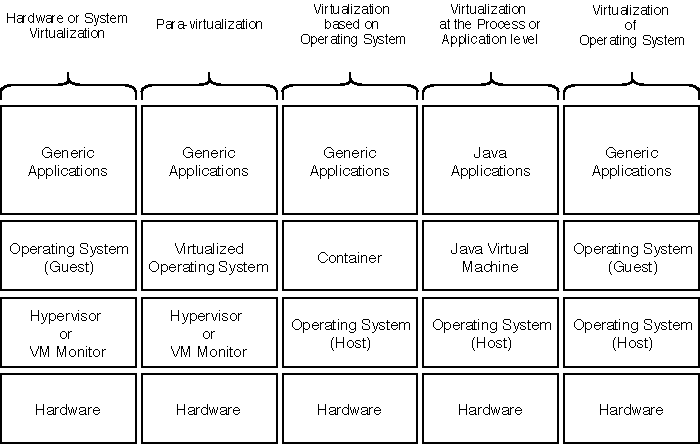
\includegraphics[width=8.5cm]{images/Pessolani2012.pdf}
		\vspace{-0.2cm}
		\caption{Taxonomy of virtual machines proposed by Pessolani et al in 2012 \cite{Pessolani2012}.}
		\label{fig:TaxonomiaDeTecnologiasDeVirtualizacion}
	\end{figure}
	
	Another way to distribute virtualization technologies is presented by \textit{Pessolani} and others in 2012 \cite{Pessolani2012}.  This study proposes a taxonomy with five main categories, such as; \textit{Hardware or System virtualization}, \textit{Para-virtualization}, \textit{Virtualization based on Operating System}, \textit{Process or application-level virtualization} and \textit{Operating system virtualization}. See Figure \ref{fig:TaxonomiaDeTecnologiasDeVirtualizacion}. Additionally, layers are also displayed for each category, suggesting a level of abstraction in which each type of virtualization takes place. The categories of this taxonomy are described below:
	
		\textbf{Hardware or system virtualization} positions the Hypervisor (Type-1) directly on top of the hardware. This is where the VMs are located with their respective operating systems' \textit{guest} to support their applications.
		
		\textbf{Para-virtualization} distributes its elements similarly to hardware or system virtualization. However, in this case the operating system \textit{guest} has been modified to be aware that it is virtualized and take advantage of its condition.
		
		\textbf{Virtualization based on operating system} is based on the use of independent workspaces called \textit{Containers}, which are based on the operating system \textit{host}. These containers allow the execution of generic applications independently.
		
		\textbf {Virtualization at the process or application level} uses an application on the host operating system to provide a VM that allows the execution of processes based on that VM. For example, JVM and Java applications.
		
		\textbf {Operating system virtualization} needs an operating system \textit{host} which carries out the functions of a hypervisor to support the operating systems \textit{guests}, which in turn have their own completely independent applications. For example \textit{User Mode Linux} \cite{Dike2006} and \textit{Minix Over Linux} \cite{Pessolani2011}.

	
	Although \textit{Pessolani}'s  taxonomy presents a summarized form of grouping virtualization technologies, it does not  explicitly consider the level of abstraction in which these technologies apply. In addition, it focuses only on the conceptual elements leaving aside specific examples. Nor does it establish a way to divide types of VMs within each main category. In addition, according to the date of publication of the study, it is necessary to carry out an update of virtualization technologies that have emerged in recent years.